\documentclass[11pt]{article}

\usepackage[a4paper, margin=2.2cm]{geometry}
\usepackage[T1]{fontenc}
\usepackage{lmodern}
\usepackage{booktabs}
\usepackage{enumitem}
\usepackage{hyperref}
\usepackage{microtype}
\usepackage{pgfplots}
\pgfplotsset{compat=1.18}

\setlist{itemsep=2pt, topsep=4pt}
\setlength{\parskip}{4pt}
\setlength{\parindent}{0pt}

\title{Few-Shot Classification with DINOv2 Embeddings\\
\large First Working Model}
\author{
    \texttt{m.mestnikov@innopolis.university}\\
    \texttt{e.moskal@innopolis.university}\\
    \texttt{k.sadykov@innopolis.university}\\
    \texttt{m.klimov@innopolis.university}
}
\date{October 2026}

\begin{document}

\maketitle

\textbf{Repository:}
\url{https://github.com/tomatoCoderq/few-shot-classification-with-dino2}

Run instructions are in \texttt{README.md}. Every number below is read from
\texttt{results/linear\_probe.csv} and \texttt{results/finetune.csv}.

\section{Data Loading and Preprocessing}

\texttt{src/data.py} downloads Oxford-IIIT Pet with
\texttt{torchvision.datasets.OxfordIIITPet} and uses the 37 breed labels.
We confirmed the sizes from the plan: 3,680 \texttt{trainval} and 3,669 \texttt{test} images.

\begin{itemize}
    \item \textbf{Test}: the official test split, used only for final metrics.
    \item \textbf{Validation}: 20 images per breed from \texttt{trainval} (740 images, seed 2026),
          used to choose $C$ for logistic regression and the epoch for fine-tuning.
    \item \textbf{Train pool}: the other 2,940 \texttt{trainval} images (at least 73 per breed).
    \item \textbf{Support sets}: $K \in \{1, 5, 10, 20\}$ images per breed from the train pool,
          for seeds 0--4. For a fixed seed the sets are nested: the $K=5$ set contains the $K=1$ set,
          so a larger $K$ only adds images.
\end{itemize}

The indices are saved in \texttt{splits/splits.json} and committed, so all members train on the
same images. Running \texttt{python -m src.data} reloads the file and fails on any overlap
between validation and train pool, any support image outside the train pool, a wrong number of
images per breed, or a broken nesting.

Preprocessing: resize the shorter side to 256, center crop $224 \times 224$, normalize with
ImageNet mean and standard deviation. The same input will go to DINOv2, since 224 is a multiple
of its patch size 14. Fine-tuning adds \texttt{RandomResizedCrop(224)} and horizontal flips to
the support images.

\section{Baseline Models}

All three runs start from torchvision ResNet-50 with \texttt{IMAGENET1K\_V2} weights and replace
the 1000-class ImageNet head with a 37-class head. They differ only in what is trained.

\begin{tabular}{@{}llrl@{}}
\toprule
ID & Trained & Parameters & Training setup \\
\midrule
E1 & linear head only & 75.8K & logistic regression on frozen embeddings \\
E5 & head + \texttt{layer4} & 15.0M & fine-tuning, BatchNorm frozen \\
E6 & whole network & 23.6M & fine-tuning, BatchNorm frozen \\
\bottomrule
\end{tabular}

\textbf{E1 (main baseline).} \texttt{src/features.py} runs the frozen backbone once over all
7,349 images and caches the 2048-d global-average-pooled embeddings. \texttt{src/linear\_probe.py}
L2-normalizes them and trains scikit-learn \texttt{LogisticRegression} (L2 penalty, lbfgs,
\texttt{max\_iter} 5000) on each support set. $C$ is chosen from $\{0.1, 1, 10, 100, 1000\}$ by
validation accuracy. A run that does not converge raises an error instead of a warning.

\textbf{E5 and E6.} \texttt{src/finetune.py}: AdamW with learning rate $10^{-3}$ for the head and
$10^{-4}$ for the backbone, weight decay $10^{-4}$, batch size 32, 30 epochs, cross-entropy.
BatchNorm stays in eval mode because a support batch is too small for reliable statistics.
After each epoch we measure validation accuracy and keep the best epoch's weights; that model
is evaluated on test once.

Every configuration runs on the same 5 support sets per $K$, so the comparison is paired.

\section{Initial Results}

\begin{tabular}{@{}lcccc@{}}
\toprule
& \multicolumn{4}{c}{Test accuracy, \% (mean $\pm$ std over 5 support sets)} \\
\cmidrule(l){2-5}
Model & $K=1$ & $K=5$ & $K=10$ & $K=20$ \\
\midrule
E1: linear head & \textbf{75.8 $\pm$ 2.3} & \textbf{87.6 $\pm$ 1.3} & \textbf{89.6 $\pm$ 0.7} & \textbf{90.9 $\pm$ 0.5} \\
E5: head + \texttt{layer4} & 50.2 $\pm$ 3.8 & 80.2 $\pm$ 0.8 & 86.5 $\pm$ 1.0 & 89.5 $\pm$ 0.7 \\
E6: whole network & 34.8 $\pm$ 2.1 & 74.7 $\pm$ 3.3 & 82.7 $\pm$ 1.0 & 86.4 $\pm$ 0.8 \\
\bottomrule
\end{tabular}

\smallskip
Macro-F1 follows accuracy within 2.6 points in every cell (E1: 74.1, 87.3, 89.4, 90.8), because
the test split has about 100 images per breed.

\begin{center}
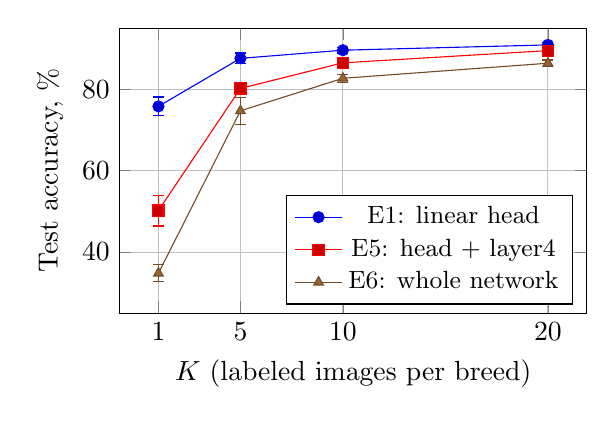
\begin{tikzpicture}
\begin{axis}[
    width=0.62\textwidth, height=5.2cm,
    xlabel={$K$ (labeled images per breed)}, ylabel={Test accuracy, \%},
    xtick={1,5,10,20}, ymin=25, ymax=95,
    legend pos=south east, legend style={font=\small}, grid=major,
]
\addplot+[mark=*, error bars/.cd, y dir=both, y explicit]
    coordinates {(1,75.8) +- (0,2.3) (5,87.6) +- (0,1.3) (10,89.6) +- (0,0.7) (20,90.9) +- (0,0.5)};
\addplot+[mark=square*, error bars/.cd, y dir=both, y explicit]
    coordinates {(1,50.2) +- (0,3.8) (5,80.2) +- (0,0.8) (10,86.5) +- (0,1.0) (20,89.5) +- (0,0.7)};
\addplot+[mark=triangle*, error bars/.cd, y dir=both, y explicit]
    coordinates {(1,34.8) +- (0,2.1) (5,74.7) +- (0,3.3) (10,82.7) +- (0,1.0) (20,86.4) +- (0,0.8)};
\legend{E1: linear head, E5: head + layer4, E6: whole network}
\end{axis}
\end{tikzpicture}
\end{center}

\begin{tabular}{@{}lll@{}}
\toprule
& Training time per run & Hardware \\
\midrule
E1 & 0.1--0.3 s, plus 88 s once to embed all images & Apple M5 (MPS, CPU) \\
E5 & 78--141 s, about 31 min for 20 runs & Kaggle NVIDIA T4 \\
E6 & 82--219 s, about 46 min for 20 runs & Kaggle NVIDIA T4 \\
\bottomrule
\end{tabular}

\smallskip
One ResNet-50 forward pass at $224 \times 224$ costs 8.17 GFLOPs (multiplies and adds counted
separately), the same for all three models.

\section{Problems and Observations}

\begin{enumerate}
    \item \textbf{The fewer parameters we train, the better the result.} E1 beats E5 and E6 at
          every $K$, by 25.6 points over E5 at $K=1$ and by 1.4 points at $K=20$. Fully fine-tuning
          23.6M parameters on 37 images loses another 15 points against E5. With this little data
          the ImageNet features are worth more than adapting them. Our main baseline for the
          DINOv2 comparison is therefore E1, and it is a strong one.
    \item \textbf{Validation is larger than the training set.} At $K=1$ a model trains on 37 images
          but selects $C$ or the epoch on 740 labeled validation images. A real few-shot user would not
          have them. The protocol is the same for all methods, so the comparison stays fair, but the
          absolute numbers are optimistic. We will report this as a limitation.
    \item \textbf{Validation overestimates test.} Validation accuracy is above test by 3.7 points
          for E5, 3.4 for E6 and 1.6 for E1. Picking the best of 30 epochs fits the validation set more
          than picking one of 5 values of $C$. We report test accuracy only.
    \item \textbf{$C$ hardly matters at $K=1$.} With one image per breed, validation accuracy changes
          by at most 0.7 points across the whole $C$ grid, so the chosen $C$ there is close to arbitrary.
          For $K \ge 5$ the choice settles on 10 or 100.
\end{enumerate}

\section{Next Steps}

E2: DINOv2 ViT-S/14 embeddings with the same logistic regression and the same support sets,
which answers the main research question against E1. Then the classifier ablations (E3, E4),
per-breed accuracy and failure cases.

\end{document}
